
%%%%%%%%%%%%%%%%%%%%%%%%%%%%%%%%%%%%%%%%%%%%%%%%%%%%%%%%%%%%%%%%%%%%%
%% This is a (brief) model paper using the achemso class
%% The document class accepts keyval options, which should include
%% the target journal and optionally the manuscript type.
%%%%%%%%%%%%%%%%%%%%%%%%%%%%%%%%%%%%%%%%%%%%%%%%%%%%%%%%%%%%%%%%%%%%%
\documentclass[journal=jpclcd,manuscript=article]{achemso}
%\documentclass[journal=jacsat]{achemso}

%%%%%%%%%%%%%%%%%%%%%%%%%%%%%%%%%%%%%%%%%%%%%%%%%%%%%%%%%%%%%%%%%%%%%
%% Place any additional packages needed here.  Only include packages
%% which are essential, to avoid problems later. Do NOT use any
%% packages which require e-TeX (for example etoolbox): the e-TeX
%% extensions are not currently available on the ACS conversion
%% servers.
%%%%%%%%%%%%%%%%%%%%%%%%%%%%%%%%%%%%%%%%%%%%%%%%%%%%%%%%%%%%%%%%%%%%%
\usepackage[version=3]{mhchem} % Formula subscripts using \ce{}

\usepackage{braket}
\usepackage{url}

\usepackage{graphicx}
\usepackage{epstopdf}


%%%%%%%%%%%%%%%%%%%%%%%%%%%%%%%%%%%%%%%%%%%%%%%%%%%%%%%%%%%%%%%%%%%%%
%% If issues arise when submitting your manuscript, you may want to
%% un-comment the next line.  This provides information on the
%% version of every file you have used.
%%%%%%%%%%%%%%%%%%%%%%%%%%%%%%%%%%%%%%%%%%%%%%%%%%%%%%%%%%%%%%%%%%%%%
%%\listfiles

%%%%%%%%%%%%%%%%%%%%%%%%%%%%%%%%%%%%%%%%%%%%%%%%%%%%%%%%%%%%%%%%%%%%%
%% Place any additional macros here.  Please use \newcommand* where
%% possible, and avoid layout-changing macros (which are not used
%% when typesetting).
%%%%%%%%%%%%%%%%%%%%%%%%%%%%%%%%%%%%%%%%%%%%%%%%%%%%%%%%%%%%%%%%%%%%%
\newcommand*\mycommand[1]{\texttt{\emph{#1}}}
\newcommand{\aglu}{\textbf{$\alpha$-Glu}}
\newcommand{\bglu}{\textbf{$\beta$-Glu}}
\newcommand{\ahct}{\textbf{$\alpha$-HCT}}
\newcommand{\bhct}{\textbf{$\beta$-HCT}}
\newcommand{\bet}{\textbf{BET}}
\newcommand{\agluahct}{\textbf{I}}
\newcommand{\bglubhct}{\textbf{II}}
\newcommand{\aglubglu}{\textbf{III}}
\newcommand{\ahctbhct}{\textbf{IV}}
\newcommand{\avib}{A_\mathrm{vib}}

%%%%%%%%%%%%%%%%%%%%%%%%%%%%%%%%%%%%%%%%%%%%%%%%%%%%%%%%%%%%%%%%%%%%%
%% Meta-data block
%% ---------------
%% Each author should be given as a separate \author command.
%%
%% Corresponding authors should have an e-mail given after the author
%% name as an \email command. Phone and fax numbers can be given
%% using \phone and \fax, respectively; this information is optional.
%%
%% The affiliation of authors is given after the authors; each
%% \affiliation command applies to all preceding authors not already
%% assigned an affiliation.
%%
%% The affiliation takes an option argument for the short name.  This
%% will typically be something like "University of Somewhere".
%%
%% The \altaffiliation macro should be used for new address, etc.
%% On the other hand, \alsoaffiliation is used on a per author basis
%% when authors are associated with multiple institutions.
%%%%%%%%%%%%%%%%%%%%%%%%%%%%%%%%%%%%%%%%%%%%%%%%%%%%%%%%%%%%%%%%%%%%%
\author{Johannes C. B. Dietschreit}
\altaffiliation{These authors contributed equally to this work}
\alsoaffiliation[CIPSM]{Center for Integrated Protein Science (CIPSM) at the Department of Chemistry, University of Munich (LMU), Butenandtstr.~5--13, D-81377 M\"unchen, Germany}
%
\author{Laurens D. M. Peters}
\altaffiliation{These authors contributed equally to this work}
\alsoaffiliation[CIPSM]{Center for Integrated Protein Science (CIPSM) at the Department of Chemistry, University of Munich (LMU), Butenandtstr.~5--13, D-81377 M\"unchen, Germany}
%
\author{J\"org Kussmann}
\alsoaffiliation[CIPSM]{Center for Integrated Protein Science (CIPSM) at the Department of Chemistry, University of Munich (LMU), Butenandtstr.~5--13, D-81377 M\"unchen, Germany}
%
\author{Christian Ochsenfeld}
\email{christian.ochsenfeld@uni-muenchen.de}
%\phone{+123 (0)123 4445556}
%\fax{+123 (0)123 4445557}
\alsoaffiliation[CIPSM]{Center for Integrated Protein Science (CIPSM) at the Department of Chemistry, University of Munich (LMU), Butenandtstr.~5--13, D-81377 M\"unchen, Germany}
\affiliation[Univerity of Munich]{Chair of Theoretical Chemistry,  Department of Chemistry, University of Munich (LMU), Butenandtstr.~7, D-81377 M\"unchen, Germany}



%%%%%%%%%%%%%%%%%%%%%%%%%%%%%%%%%%%%%%%%%%%%%%%%%%%%%%%%%%%%%%%%%%%%%
%% The document title should be given as usual. Some journals require
%% a running title from the author: this should be supplied as an
%% optional argument to \title.
%%%%%%%%%%%%%%%%%%%%%%%%%%%%%%%%%%%%%%%%%%%%%%%%%%%%%%%%%%%%%%%%%%%%%
\title{Identifying Free Energy Hot-Spots\\ in Molecular Transformations}

%%%%%%%%%%%%%%%%%%%%%%%%%%%%%%%%%%%%%%%%%%%%%%%%%%%%%%%%%%%%%%%%%%%%%
%% Some journals require a list of abbreviations or keywords to be
%% supplied. These should be set up here, and will be printed after
%% the title and author information, if needed.
%%%%%%%%%%%%%%%%%%%%%%%%%%%%%%%%%%%%%%%%%%%%%%%%%%%%%%%%%%%%%%%%%%%%%
\abbreviations{DoS, Glu, HTC}
\keywords{Free Energy, Local Effects, Anomeric Effect, Binding Event}


\begin{tocentry}
	\centering
	\large
	Finding Free Energy Hot-Spots
	
	\vspace{1.5ex}
	
	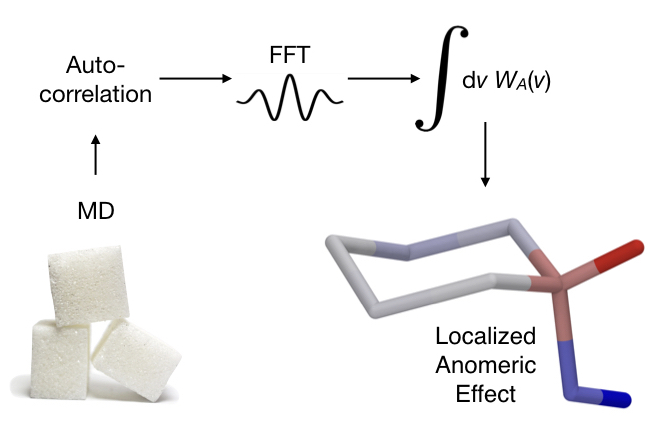
\includegraphics[width=5cm]{TOC}
	
\end{tocentry}

\begin{document}
%%%%%%%%%%%%%%%%%%%%%%%%%%%%%%%%%%%%%%%%%%%%%%%%%%%%%%%%%%%%%%%%%%%%%
%% The manuscript does not need to include \maketitle, which is
%% executed automatically.  The document should begin with an
%% abstract, if appropriate.  If one is given and should not be, the
%% contents will be gobbled.
%%%%%%%%%%%%%%%%%%%%%%%%%%%%%%%%%%%%%%%%%%%%%%%%%%%%%%%%%%%%%%%%%%%%%
\begin{abstract}
 The free energy is one of the central quantities in material and natural sciences. While being well-established, e.g., in drug design or catalyst optimization, computational methods lack a straightforward way to gain deeper insights into the calculated free energy, and thus the underlying chemical or physical processes. Here, we present a generally applicable, spectrum-based ansatz that tackles this shortcoming by identifying contributions from specific atoms or groups to the free energy. We illustrate this in studies of the bromodomain-inhibitor binding and the anomeric effect in glucose providing quantitative evidence in line with chemical intuition in both cases. For the latter example we also report an experimental infrared spectrum and find excellent agreement with our simulated spectra.
\end{abstract}

%%%%%%%%%%%%%%%%%%%%%%%%%%%%%%%%%%%%%%%%%%%%%%%%%%%%%%%%%%%%%%%%%%%%%
%% Start the main part of the manuscript here.
%%%%%%%%%%%%%%%%%%%%%%%%%%%%%%%%%%%%%%%%%%%%%%%%%%%%%%%%%%%%%%%%%%%%%
The free energy is the driving force behind every chemical reaction. It determines, for example, the rate of an enzymatic reaction or the scope of products formed during a catalytic reaction. The prediction of free energies is, therefore, a key challenge in modern quantum chemistry\cite{Chipot2007,Hansen2014}. For small systems this is usually done via a frequency analysis at quantum mechanics (QM) level of theory, while free energy differences of larger systems are determined from sampled energies along Monte Carlo\cite{Metropolis1953,Hastings1970} or molecular dynamics (MD)\cite{Fermi1955,Alder1959,Rahman1964} simulations applying, e.g., exponential averaging theory\cite{Zwanzig1954} or Bennett's acceptance ratio method\cite{Bennett1976}.

While the mentioned methods have been used extensively in different fields\cite{Rickman2002,Karplus1990,Gao1989,Bash1987a}, the interpretation of their results is in most cases not straightforward. The reason for this is that it is not always possible to separate the free energy change into contributions from different interactions, atoms, or residues so that the following key questions cannot be answered:

\begin{enumerate}
	\item[Q1.] Which atoms or residues are affected by the transformation, and therefore contribute to the free energy change?
	\item[Q2.] Which effects (e.g., bond weakening, sterical clashes, new non-covalent interactions) cause the free energy change?
	\item[Q3.] Can we quantify these atom- or residue-wise contributions?
\end{enumerate}

Applying the conventional energy-based methods\cite{Zwanzig1954,Bennett1976}, some form of fragmentation is possible for simple force fields\cite{Gao1989,Irwin2018}, however, this is not possible when non-additive force fields (like the emerging polarisable force fields\cite{Baker2015}), QM calculations, or combined quantum mechanics/molecular mechanics (QM/MM) calculations are used.

Thus, the main idea in this work is to extract the free energy from the velocities ($\mathbf{v}_j$) of each atom $j$ during a molecular dynamics simulation. This is done by calculating the density of state function ($D(\nu)$) as the Fourier transform of the velocity autocorrelation function
%
\begin{equation}
D(\nu) = 2 \beta \sum \limits_{j = 1}^{N} m_j \int dt
\braket{\mathbf{v}_j (\tau) \mathbf{v}_j (t + \tau)}_{\tau} e^{-i 2\pi \nu t}.
\label{eq1}
\end{equation}
%
$\beta$ is equal to $1/(k_\mathrm{B} T)$ with $k_\mathrm{B}$ being the Boltzmann constant and $T$ the absolute temperature. $m_j$ is the mass of atom $j$ and $N$ is the total number of nuclei. The free energy ($A$) can then be calculated from a weighted integral over the frequency ($\nu$)
%
\begin{equation}
A = E + \avib{} = E + \beta^{-1} \int_{0}^{\infty} d\nu D(\nu) \ln [\beta h \nu]\ ,
\label{eq2}
\end{equation}
%
with $E$ being the potential energy at the minimum energy geometry and $h$ the Planck constant. While the mathematics have originally been introduced by Berens \textit{et al.}\cite{Berens1983} to estimate quantum corrections to thermodynamic properties, it has, to our knowledge, not been used to calculate or interpret free energy differences of molecular transformations. For a more detailed analysis of the contributions to $A$ and its connection to the Gibbs free energy ($G$), the reader is referred to the Supporting Information.  

Equations~\ref{eq1} and \ref{eq2} indicate that $\avib{}$ can be split into contributions from the individual nuclei, as $D(\nu)$ is calculated as a sum over all atoms (see Methods section for details). Consequently, the method delivers answers to the questions Q1 and Q3 directly. Question Q2 can be addressed indirectly by evaluating $D(\nu)$ itself. We make the reasonable assumption that the local changes in $\avib{}$ occur foremost at those sites which cause $A$ to change.

As a first demonstration of this approach, we investigate the change of $\avib{}$ during the binding of a bromodomain-containing protein to an inhibitor. Proteins of the bromo- and extra-terminal domain (\bet{}) family are involved in the recognition of acetylated lysine residues and play an important role in epigenetic communication\cite{Filippakopoulos2012}. Very recently, potent mutant-selective inhibitors for \bet{} have been developed\cite{Runcie2018}, which are meant as a tool for future \textit{in vivo} studies. Upon binding to the inhibitor, the potential energy surface of \bet{} is modified leading to conformational changes in the protein which one would generally assume causes the binding site to become tighter.

We used the co-crystal structure of \textbf{9-ME-1} and \bet{} as well as the apo-crystal structure (PDB 5O3C and 5O38\cite{Runcie2018}) as a starting point to investigate the effect of inhibitor binding to the bromodomain motif. We conducted two independent classical molecular dynamics simulations and computed the difference in vibrational free energy ($\Delta \avib{}$) per residue and per atom (for full details see the Materials and Methods section in the Supporting Information). The changes in the vibrational free energy are shown in Fig.~\ref{fig:bromo}. Blue indicates a stiffening of the residue ($\Delta \avib{} > 0$) upon the binding of the inhibitor ("cold" regions), whereas red ($\Delta \avib{} < 0$) means that the residue can move more freely ("hot" regions).

\begin{figure*}[h!]
	\centering
	\includegraphics[width=16cm]{fig1.eps}
	\caption{%\textbf{Visualizing the binding of the bromodomain with an inhibitor.} 
		\textbf{a}, Changes of the vibrational free energy ($\Delta \avib{}$) within the bromodomain upon binding the inhibitor. The residues are coloured according to the changes in $\avib{}$ going from the apo- to the complexed-form. Blue ("cold") residues indicate a gain in vibrational free energy ($\Delta \avib{} > 0$, less movement) and red ("hot") residues indicate a loss in vibrational free energy ($\Delta \avib{} < 0$, more freedom). The inhibitor is shown with vdW-spheres coloured according to atom types. 
		\textbf{b}, Interaction between the residues and the inhibitor. TRP-26 (van-der-Waals interaction), TYR-42 (hydrogen bond), and CYS-81 (two hydrogen bonds) are highlighted.  
		\textbf{c}, Interactions within the helical part of the domain. }
	\label{fig:bromo}
\end{figure*}

The overall change in $\Delta \avib{}$ (+35.2~kJ/mol) indicates a stiffening of the motif due to the interaction with the inhibitor. Many of those "cold" residues can be found in the binding pocket (see  Fig.~\ref{fig:bromo}a+b), where their sidechains show distinct interactions with the inhibitor. Examples are TRP-26, which interacts with the inhibitor via van-der-Waals interactions, and TYR-42, which forms a hydrogen bond. Interactions between the inhibitor and the backbone are also occurring. The peptide group of LYS-30, for example, communicates with \textbf{9-ME-1} via a water molecule. The only "hot" residue in the binding pocket is CYS-81, whose SH-group switches between two hydrogen bond acceptors (one at \bet{} and one at the inhibitor). Both hydrogen bonds cannot be formed in the apoprotein. The analysis, however, also shows that $\avib{}$ does not only change at the binding site, as parts of the $\alpha$-helices are coloured as well (see Fig.~\ref{fig:bromo}c). Reasons for these significantly smaller contributions are subtle changes in the arrangement of the helices.

A general mode softening (increase of the density of states function for very small wave numbers) as reported in experimental measurements\cite{2004Balog} and normal mode analysis\cite{2010Moritsugu} was not found in the present study. As we have shown elsewhere\cite{Peters2018}, normal mode analysis is not as flexible as the density of states method. The residues inside the binding pocket show a clear stiffening and there are no new soft modes. However, there are about 20~\% of the residues that exhibit new soft modes for the inhibitor-protein complex. All of these residues have side chains that are facing away from the inhibitor towards the solvent. The increase in slow modes are caused by the loss of rotational and translational modes of the inhibitor that are transferred onto the protein upon binding as additional vibrational modes as well as the coupling of modes from inhibitor and protein.\cite{2010Moritsugu}

\begin{figure*}[h!]
	\centering
	\includegraphics[width=16cm]{fig2.eps}
	\caption{%\textbf{Visualizing the anomeric effect in glucose}.
		\textbf{a}, (top) Hyperconjugation and (bottom) dipole interaction as origins of the anomeric effect in glucose.
		\textbf{b}, Structures, abbreviations, and atom labels of the investigated molecules. The possible transformations \textbf{I} to \textbf{IV} are aranged in a thermodynamic cycle.
		\textbf{c}, Change in the vibrational free energy per atom from \bglu{}$\rightarrow$\bhct{} (transformation \bglubhct{}), \aglu{}$\rightarrow$\ahct{} (transformation \agluahct{}), and their difference (\bglubhct{}-\agluahct{} = \ahctbhct{}-\aglubglu{}). The latter is equivalent to the change of the free energy during the appearance of the anomeric effect reflecting the bond strengthening of the O5-C1 bond and the bond weakening of the C1-O1 and C5-O5 bond.
	}
	\label{fig:glucose}
\end{figure*}


In the first example we focused on intermolecular interactions, but our method can also visualise changes of covalent bonds. Therefore, we use, as a second example, \emph{ab initio} molecular dynamics instead of force field calculations (see the Supporting Information for full details) to investigate the anomeric effect, which explains the stabilization of $\alpha$-glucose (\aglu{}) with respect to $\beta$-glucose (\bglu{}). Its origin (hyperconjugation and/or dipole interactions) has been under discussion for a long time including experimental\cite{Cocinero2011} as well as theoretical\cite{Mo2010} contributions (see Fig.~\ref{fig:glucose}a). Here, we restrict ourselves to the visualization of its effect without discussing its origin.


The sole comparison of \aglu{} and \bglu{} would not only incorporate the anomeric but also other effects, for example, changes of the hydrogen bonds or the 1,3-diaxial interactions. To isolate and visualize the anomeric effect, we have simulated \aglu{}, \bglu{}, and their two analogues with the ring oxygen being replaced by a CH$_2$ moiety (\ahct{} and \bhct{}, the abbreviation \textbf{HCT} stands for the IUPAC name 5-\textbf{H}ydroxymethyl-\textbf{c}yclohexane-(1,2,3,4)-\textbf{t}etrole) at HF-3c\cite{Sure2013} level of theory. Please note that the anomeric effect is only present in \aglu{}. It can, therefore, be investigated by analysing the difference between the transformations \aglu{}$\rightarrow$\ahct{} (\agluahct) and \bglu{}$\rightarrow$\bhct{} (\bglubhct) or between the transformations \aglu{}$\rightarrow$\bglu{} (\aglubglu) and \ahct{}$\rightarrow$\bhct{} (\ahctbhct), as the other effects cancel out. For structures and atomic labels see Fig.~\ref{fig:glucose}b.

\begin{figure*}[h!]
	\centering
	\includegraphics[width=16cm]{fig3.eps}
	\caption{%\textbf{Detailed analysis of the C-H stretching vibrations.} 
		\textbf{a}, Excerpt of the experimental IR-spectrum of crystalline glucose (mono-hydrate and mixture of the $\alpha$- and $\beta$-anomer) showing the C-H stretching vibrations for comparison to the simulated spectra below.
		\textbf{b}, Labels of carbon atoms in \aglu{}, \bglu{}, \ahct{}, and \bhct{}.
		\textbf{c}, Calculated spectra ($D(\nu)$) of (top) \aglu{} and (bottom) \bglu{} showing the C-H stretching vibrations of the entire molecule (black) and the contributions from the different C-H bonds (colour). The splitting of molecular peaks enables a detailed inspection of the surroundings of the individual atoms. For comparison to the experiment, the simulated spectra have been scaled by a factor of $0.82$ (similar to the reported $0.81$\cite{Peters2017}).
		\textbf{d}, Same analysis for (top) \ahct{} and (bottom) \bhct{}. The peaks of H7 and H7' (around 3050~cm$^{-1}$) are not shown as they cannot be compared to glucose.}
	\label{fig:hydrogen_bonds}
\end{figure*}

The free energy changes of the entire molecules ($\Delta A$(\aglubglu{}) $ = + 7.91$ kJ/mol; $\Delta A$(\ahctbhct{}) $ = + 3.04$ kJ/mol) already indicate the occurrence of the anomeric effect in our simulations. In order to visualise it, we show the vibrational free energy differences ($\Delta \avib{}$) of the transformations \agluahct{} and \bglubhct{} for selected atoms in Fig.~\ref{fig:glucose}c (for the corresponding vibrational spectra see SFig.~(1) ). Their difference, which can be interpreted as the appearance of the anomeric effect, is also shown. In both transformations (\agluahct{} and \bglubhct{}), the centres near the mutation site C7/O5 and (in the case of \agluahct{}) O1 contribute to $\Delta \avib{}$, whereas C2-4 are not affected by the mutation. Their difference (\bglubhct{} - \agluahct{}) reveals that $\Delta \avib{}$ of the anomeric effect is mainly localised at C1, O1, and their hydrogen atoms as well as at C5 and O5. It is in good agreement with the bond strengthening of the O5-C1 bond (C1 is red) and the bond weakening of the C1-O1 bond (O1 is blue), when the anomeric effect appears. Additionally, the C5-O5 bond is slightly weakened (C5 is blue). The comparably small contribution at O5 is the result of two counteractive effects, the simultaneous strengthening and weakening of its bonds to C1 and C5, respectively. All effects are also visible in the distributions of bond lengths during the simulations (see SFig.~(2) ). 



The C-H stretching vibrations of the systems (Fig.~\ref{fig:hydrogen_bonds}) can also be used to visualise the anomeric effect, as they are very good sensors for changes in the surrounding chemical environment. The superposition spectra of \aglu{} and \bglu{} (black lines in Fig.~\ref{fig:hydrogen_bonds}c) are in good agreement with the experimental infrared spectrum measured in the present work (Fig.~\ref{fig:hydrogen_bonds}a) featuring both six peaks. Comparing \aglu{} and \bglu{} (Fig.~\ref{fig:hydrogen_bonds}c), we can identify two red-shifts (C1-H1 and C5-H5), which do not appear in the \textbf{HCT}-spectra (Fig.~\ref{fig:hydrogen_bonds}d). They can, therefore, be assigned to the anomeric effect corroborating the previous result that the anomeric effect affects the vibrations of C1, C5, and O1 as well as the connected hydrogen atoms and not C2-C4 and C6.


Overall, the use of vibrational spectra calculated from nuclear velocities, can lead to new and valuable insights into molecular transformations. As the two examples have shown, we are able to localize, explain, and quantify free energy changes, and therefore answer the three key questions posed at the beginning of this work. Our results are in absolute agreement with chemical intuition for which our method provides a solid, quantifiable, and generally valid fundament. We suggest that this ansatz should be used, e.g, in drug or catalyst design, in addition to the calculation of energies and the investigation of structural parameters to gain the full picture of the problem at hand. 






%%%%%%%%%%%%%%%%%%%%%%%%%%%%%%%%%%%%%%%%%%%%%%%%%%%%%%%%%%%%%%%%%%%%%
%% The "Acknowledgement" section can be given in all manuscript
%% classes.  This should be given within the "acknowledgement"
%% environment, which will make the correct section or running title.
%%%%%%%%%%%%%%%%%%%%%%%%%%%%%%%%%%%%%%%%%%%%%%%%%%%%%%%%%%%%%%%%%%%%%
\begin{acknowledgement}

The authors acknowledge Sophia Schwarz and Oliver Trapp (LMU Munich) for their help in measuring the experimental infrared spectrum, and Henry Fritz Schaefer III (University of Georgia, Athens, USA) for useful comments on our manuscript.
%
%
Financial support was provided by the SFB 749  "{}Dynamik und Intermediate molekularer Transformationen"{} (DFG), the DFG cluster of excellence (EXC 114) "{}Center for Integrative Protein Science Munich"{} (CIPSM), and the Innovative Training Network "{}Computational Spectroscopy In Natural Sciences And Engineering"{} (ITN-COSINE). C.O. acknowledges further support as Max-Planck-Fellow at the MPI-FKF Stuttgart.

\end{acknowledgement}

%%%%%%%%%%%%%%%%%%%%%%%%%%%%%%%%%%%%%%%%%%%%%%%%%%%%%%%%%%%%%%%%%%%%%
%% The same is true for Supporting Information, which should use the
%% suppinfo environment.
%%%%%%%%%%%%%%%%%%%%%%%%%%%%%%%%%%%%%%%%%%%%%%%%%%%%%%%%%%%%%%%%%%%%%
\begin{suppinfo}

Additional analysis and figures can be found in the Supplementary Information.

\end{suppinfo}

%%%%%%%%%%%%%%%%%%%%%%%%%%%%%%%%%%%%%%%%%%%%%%%%%%%%%%%%%%%%%%%%%%%%%
%% The appropriate \bibliography command should be placed here.
%% Notice that the class file automatically sets \bibliographystyle
%% and also names the section correctly.
%%%%%%%%%%%%%%%%%%%%%%%%%%%%%%%%%%%%%%%%%%%%%%%%%%%%%%%%%%%%%%%%%%%%%
\bibliography{nature}

%%%%%%%%%%%%%%%%%%%%%%%%%%%%%%%%%%%%%%%%%%%%%%%%%%%%%%%%%%%%%%%%%%%%%
%% The "tocentry" environment can be used to create an entry for the
%% graphical table of contents.
%%%%%%%%%%%%%%%%%%%%%%%%%%%%%%%%%%%%%%%%%%%%%%%%%%%%%%%%%%%%%%%%%%%%%


\end{document}
